% Created 2023-01-02 lun 11:20
% Intended LaTeX compiler: pdflatex
\documentclass[openany, a4paper]{book}
\usepackage[utf8]{inputenc}
\usepackage[T1]{fontenc}
\usepackage{graphicx}
\usepackage{longtable}
\usepackage{wrapfig}
\usepackage{rotating}
\usepackage[normalem]{ulem}
\usepackage{amsmath}
\usepackage{amssymb}
\usepackage{capt-of}
\usepackage{hyperref}
\usepackage{amsmath,amssymb,amsthm,geometry,hyperref,paralist,svg,thmtools,tikz,tikz-cd}
\usepackage[spanish]{babel}
\usepackage{mathtools}
\usepackage[capitalise,noabbrev]{cleveref}
\usepackage{mdframed} \usepackage{svg}
\usepackage{environ} \NewEnviron{abmn}{\marginnote{\BODY}}
\usepackage{url}
\usepackage{color}
\usepackage{listings,chngcntr}% http://ctan.org/pkg/listings
\usepackage{multicol}
\usepackage{url}
\lstset{ basicstyle=\ttfamily, mathescape=true, frame=Trbl, numbers=left}
\renewcommand{\thelstlisting}{\thesection.\arabic{lstlisting}}
\renewcommand{\lstlistingname}{Pseudocódigo}
\counterwithin{lstlisting}{section}
\setcounter{tocdepth}{1}
\newtheoremstyle{break}{\topsep}{\topsep}{\itshape}{}{\bfseries}{}{\newline}{}
\theoremstyle{break}
\newtheorem{theorem}{Theorem}
\newtheorem{corollary}[theorem]{Corollary}
\newtheorem{proposition}[theorem]{Proposition}
\newtheorem{definition}[theorem]{Definition}
\newtheorem{lemma}[theorem]{Lemma}
\newtheorem{affirmation}[theorem]{Affirmation}
\theoremstyle{example}
\newtheorem{example}{Example}
\newtheorem{exmpl}{Example}
\theoremstyle{note}
\newtheorem{note}{Note}
\theoremstyle{break}
\newtheorem{remark}{Remark}
\theoremstyle{exercise}
\newtheorem{exercise}{Exercise}
\usetikzlibrary{arrows,automata,positioning}
\NewEnviron{obs}{\begin{mdframed}\begin{remark} \BODY \end{remark}\end{mdframed}}
\NewEnviron{nota}{\begin{mdframed}\begin{note} \BODY \end{note}\end{mdframed}}
\renewcommand{\qedsymbol}{\textbf{\therefore}}
\NewEnviron{myproof}[1][\proofname]{\begin{proof}[#1]$ $\par\nobreak\ignorespaces}{\end{proof}}
\NewEnviron{blk}{\begin{mdframed}\BODY\end{mdframed}}
\newcommand{\nimplies}{\;\not\nobreak\!\!\!\!\implies}
\author{Miguel Angel Piña Avelino}
\date{\today}
\title{Notes about concurrent computing}
\hypersetup{
 pdfauthor={Miguel Angel Piña Avelino},
 pdftitle={Notes about concurrent computing},
 pdfkeywords={},
 pdfsubject={},
 pdfcreator={Emacs 28.2 (Org mode 9.5.5)},
 pdflang={Spanish}}
\begin{document}

\maketitle
\tableofcontents


\part{Introduction}
\label{sec:orga341d6c}

\chapter{Work-stealing algorithm analysis}
\label{sec:orga263b2b}

We analyze the algorithms for work-stealing described in the article Fully
Read/Write Fence Free Work-Stealing With Multiplicity, also the algorithm
called "Idempotent FIFO Work-Stealing", this because the algorithm have a
similar semantic than the prior algorithms.

\section{Realistic model of computation}
\label{sec:orgf55372b}

We consider a standard concurrent shared memory system with \(n \ge 2\)
\emph{asynchronous} processes, \(p_0, \ldots, p_{n-1}\), which may crash at any time
during an execution. The processes communicate with each other by invoking
atomic instructions of base objects: either simple Read/Write instructions to
\textbf{atomic objects}, or more powerful \textbf{Read-Modify-Write} instructions, such as
\texttt{Test-And-Set}, \texttt{Swap} or \texttt{Compare-And-Set}.

For simplicity we assume a single multicore chip where the processes run. In
our system we consider a memory hierarchy, where we have the following
elements in the hierarchy:

\begin{itemize}
\item Cache memory
\item Memory bus
\item Main memory
\end{itemize}

In this model, each processor core may read and
write to a single shared memory space. Usually each processor core has a
cache to operate with data from the shared memory. Often, this data is
transferred through a memory bus, allowing connect the processors with the
memory. The figure \ref{fig:arch} shows a simplified view of this model. In
the sections: \hyperref[sec:org019acd5]{Cache memory}, \hyperref[sec:org53c2095]{Memory bus} and \hyperref[sec:orge0946a4]{Main memory}, we explain more in
detail the meaning of each bullet of the list.

\begin{figure}
\begin{minipage}{\linewidth}
  \includesvg[width=\linewidth]{architecture}
\end{minipage}
\caption{Simplified view of a modern computer system cache architecture}
\label{fig:arch}
\end{figure}

\section{Cache memory}
\label{sec:org019acd5}

The cache memory is a special very high-speed memory that is very close to
the processor and the processes can access it very fast. The caches are used
to reduce average latencies to access storage structures
\cite{DBLP_series_synthesis_2020Nagarajan}. In recent multicore chips, the
cache memory is divided in three levels, two private levels (L1 and L2) for
each processor and a third level (L3) that is shared by the cores. The
purpose of the first two levels is to provide fast access to data and
instructions for the processors.

Each processor use the first level of cache to get the data and instructions
to execute them, usually the access to this level of cache is very fast
respect to the access to other levels.  The second level is often more
capacious than first level and is used to store data and instructions that
are close to be executed. In the third level, this cache is shared by many
processors and is used as feeder for the L2 cache.


\section{Memory bus}
\label{sec:org53c2095}

Is a computer bus that allows transfer data from the primary memory to the
CPU and the cache memory. It is made up of two parts: the data bus and the
address bus. The data bus is in charge of transfer information between the
primary memory and the correspondent chipset.
The address bus is used to retrieve information about the location of stored
information.


\section{Main memory}
\label{sec:orge0946a4}

Is the responsible of hold the data that CPU need to access frequently, such
as instructions or data currently being processed. The CPU can access to
this information faster than the access to secondary memory.

\section{Consistency Memory Model and Cache Coherence}
\label{sec:org2c44494}

\begin{enumerate}
\item Consistency memory model
\label{sec:orgd8a9a59}

Following the simplified view of the cache architecture, we want to have a
correct shared memory. And what this means? The correctness of the shared
memory can be separated into two sub-issues: \emph{consistency} and \emph{correctness}.

The consistency (definitions) provide rules about loads and stores (memory
reads and writes) and how they act upon memory. These definitions must take
into account the behaviour of those operations on memory through access of
multiple threads or even a single thread. The consistency models define
correct shared memory behavior in terms of loads and stores, without
reference to caches or coherence \cite{DBLP_series_synthesis_2020Nagarajan}.
Shared memory correctness is specified by a memory consistency model (or
memory model). This specifies the allowed behavior of multithreaded programs
executing with shared memory.

The most intuitive and strongest memory model is the \emph{Sequential Consistency}
(SC). Another memory model used by systems \emph{x86} and \emph{SPARC} is \emph{Total Store Order}
(TSO), motivated by the desire of use \emph{first-in-first-out} write buffers to
hold the results of committed stores before writing results to the caches.
Additional to the prior memory model, "relaxed" or "weak" memory models are
considered, because these models shows that most memory orderings in strong
models are unnecessary \cite{DBLP_series_synthesis_2020Nagarajan}.

\item Cache coherence
\label{sec:orgc5cbfb9}

Cache coherence protocols are used in response to solve a coherence problem
in cache. For example, a coherence problem can arise if multiple cores have
access to multiple copies of a datum, each one in a core, and at least one
them is a write access. The cache coherence protocols prevent the access to
stale data (incoherent data); this can be done using a set of rules
implemented by the distributed set of cores within a system. These
protocols use the common MOESI coherence states: modified (M), owned (O),
exclusive (E), shared (S) and invalid (I). The protocol acts like a state
machine, moving from one state to another based on the conditions of the
data and the cache memory \cite{DBLP_series_synthesis_2020Nagarajan}.
\end{enumerate}

\section{Memory fences}
\label{sec:orgacf7b47}

A memory fence is a barrier instruction that causes a CPU or compiler to
enforce a an ordering constraint on memory operations (loads and stores)
issued before and after the barrier instruction.

These instructions are necessary because most modern CPUs or compilers
employ performance optimizations, changing the order of the instructions on
one program, that could result in out-of-order execution. Normally these
optimizations are unnoticed in a single thread program, but can cause an
unpredictable behavior in concurrent programs.

For example, consider the following multi-thread program, with 2
threads, each one running in one core in a concurrent way:

Thread 1, core 1
\begin{verbatim}
while (z == 0);
print(y);
\end{verbatim}

Thread 2, core 2
\begin{verbatim}
y = 30;
z = 1;
\end{verbatim}

In this case, we might expect that the \texttt{print(y)} always print the number 30,
nevertheless, the compiler or the CPU could change the order of the
instructions for the thread 2, giving as result an execution where the value
for \texttt{y} is undefined and the instructions could be interleaved as follows:

\begin{verbatim}
z = 1; // Thread 2
while (z == 0); // Thread 1
print(y); // Thread 1
y = 30; // Thread 2
\end{verbatim}

This execution is sequentially consistent, but is an out-of-order
execution producing an undefined result. With the use of memory barriers, we
can ensure that instructions don't be reordered. For example, our code could
be rewrite as follows:

Thread 1, core 1.
\begin{verbatim}
while (z == 0);
fence()
print(y);
\end{verbatim}

Thread 2, core 2.
\begin{verbatim}
y = 30;
fence();
z = 1;
\end{verbatim}


Languages as \texttt{Java} or \texttt{C++} provide instructions to establish synchronization
and ordering constraints between threads without an atomic operation. These
instructions have semantics well defined for

In the case of Java, we have static methods of the class VarHandle
(\texttt{java.lang.invoke.VarHandle}) that are refered as memory fence methods which
helps to provide fine-grained control of memory ordering. These statics
methods are \cite{varHandleJdk92017}:

\begin{description}
\item[{fullFence}] Ensures that loads and stores before the fence will not be
reordered with loads and stores after the fence. This method has memory
ordering effects compatible with
\texttt{atomic\_thread\_fence(memory\_order\_seq\_cst)}.
\item[{acquireFence}] Ensures that loads before the fence will not be reordered
with loads and stores after the fence. This method has memory ordering
effects compatible with \texttt{atomic\_thread\_fence(memory\_order\_acquire)}.
\item[{releaseFence}] Ensures that loads and stores before the fence will not
be reordered with stores after the fence. This method has memory ordering
effects compatible with \texttt{atomic\_thread\_fence(memory\_order\_release)}.
\item[{loadLoadFence}] Ensures that loads before the fence will not be
reordered with loads after the fence.
\item[{storeStoreFence}] Ensures that stores before the fence will not be
reordered with stores after the fence.
\end{description}

For C++, we have the function
\texttt{std::atomic\_thread\_fence}\cite{threadFenceCpp2020}, which establishes
memory synchronization ordering of non-atomic and relaxed atomic access, as
instructed by order, without an associated atomic operation. The type of
synchronization that can handle are the following:

\begin{itemize}
\item Fence-atomic synchronization
\item Atomic-fence synchronization
\item Fence-Fence Synchronization
\end{itemize}

And using a memory order\cite{memoryOrderCpp2020}, it can specifies how
memory accesses, including regular, non atomic memory accesses, are to be
ordered around an atomic operation. In total are six orders, from the
relaxed memory order to the sequential consistent memory order. They are:
\texttt{memory\_order\_relaxed}, \texttt{memory\_order\_consume}, \texttt{memory\_order\_acquire},
\texttt{memory\_order\_acq\_rel} and \texttt{memory\_order\_seq\_cst}. A note about
\texttt{atomic\_thread\_fence} functions, is that on x86 (x86\textsubscript{64}), these functions
issue no CPU instructions and only affect compile time code, with exception
for \texttt{std::atomic\_thread\_fence(std::memory\_order::seq\_cst)}, which issue the
full memory fence instruction \texttt{MFENCE}. For other archict

\section{Pseudocode for Work-Stealing with Weak Multiplicity}
\label{sec:org2b85b72}



\chapter{Some Foundations}
\label{sec:orgd689933}

\section{Cache memory}
\label{sec:org1a81cdd}

The cache memory

\begin{enumerate}
\item Multiple caches
\label{sec:orge00887a}


\item Cache coherence protocols
\label{sec:orgacbc1db}



\begin{enumerate}
\item MESI
\label{sec:orgcbdd74c}


\item MOESI
\label{sec:org4630fa7}
\end{enumerate}


\item Store Buffers
\label{sec:org6ce038f}
\end{enumerate}


\section{Reordering (CPU or Compiler)}
\label{sec:org6e18f2e}


\section{Memory Barriers}
\label{sec:org8800593}


\begin{enumerate}
\item X86 and TSO architectures
\label{sec:orgeaedeef}


\item Memory Fences
\label{sec:org52424a3}
\end{enumerate}


\section{Read-Modify-Write Operations}
\label{sec:orga68e2ef}


\section{Bibliography}
\label{sec:org6fcba64}

\begin{itemize}
\item \url{https://blog.the-pans.com/std-atomic-from-bottom-up/}
\end{itemize}


\section{Memory management}
\label{sec:orgc8c5cde}

To implement efficiently the idempotent algorithms in an enviroment without
garbage collection, it's necessary use some technique or metodology to
provide garbage collection when atomic pointers are used or when distinct
threads want to reclaim the memory of the object associated to the pointer.

\begin{enumerate}
\item Strategies to delete shared pointers
\label{sec:org1d28632}

\begin{itemize}
\item Add pointers to list to safety delete.
\item Do this when there aren't more threads accessing to methods.
\begin{itemize}
\item Increase the counter when a thread enter to the method and decrease when
it exits.
\item Delete all pointers when the counter be equal to zero.
\end{itemize}
\end{itemize}


\item Hazard pointers
\label{sec:orgccc3eb8}

The \emph{Hazard Pointers} is a technique to manage memory in languages where there
are not a garbage collector. This technique was proposed by Maged
Michael \cite{DBLP_journals_tpds_Michael04}. They are so called because
deleting a pointer that might be referenced by other thread(s) is
dangerous. If another threads keep holding references to that pointer and
proceed to access to that pointer after be deleted, you have a undefined
behavior \cite{DBLP_journals_tpds_Michael04}.

The basic idea of this technique is the following:

\begin{itemize}
\item If a thread want to use a pointer that another thread might want to
delete, it first sets a hazard pointer to the pointer, informing to the
other thread that deleting the pointer would be dangerous. Once the object
is not longer needed, the hazard pointer is cleared.
\item When a thread wants to delete the pointer, it must check if the hazard
pointers belonging to the other threads in the system. If no one has a
reference to the pointer, then, it's safe to delete the
pointer. Otherwise, it must be left until later.
\item Periodically, we must check the list of objects that have been left until
later to see if any of them can be deleted now.
\end{itemize}

A general pseudocode for this technique could be the following:

\begin{verbatim}
void func() {
    std::atomic<void*>& hp = get_hazard_pointer_for_current_thread();
    void* old_data = data.load();
    do {
        void* temp;
        do{ // Loop until you've set the hazard pointer
            temp = old_data;
            hp.store(old_data);
            old_data = data.load();
        } while (old_data != temp);
          }while (old_data &&
            !data.compare_exchange_strong(old_data, old_data->next);
    // Do something with old_data
    hp.store(nullptr); // clearing usage of hazard pointer
    // Trying clearing
    if (outstanding_hazard_pointers_for(old_head))
    {
        reclaim_later(old_data);
    }
    else
    {
        delete old_data;
    }
    delete_nodes_with_no_hazards();
}
\end{verbatim}


\item Atomic Smart Pointers (Herlihy, Chapter 19) (Not available for GCC and CLang)
\label{sec:orgc092189}


When a memory region is reclaimed, the programmer cannot know how that
region of memory will be reused or if even whether it is reused. We need a
way of developing a (general) solution to prevent the sorts of races
when a memory region is reclaimed by many threads asynchronously. We can to
do this by delaying reclamation.
Thinking in terms of pending operations on a concurrent data structure, a
sufficient condition is that \emph{memmory is only reclaimed when it is impossible
for any pending operation to access in the future}.

This property could be also achieved by \emph{reference counting}. In a reference
counted implementation of a data-structure (like a list), a counter of type
atomic<int> is associated with each node. Whenever a reference to node N is
created
\end{enumerate}


\chapter{Memory management for work-stealing algorithms}
\label{sec:org8701a1a}

It is well known that C++ does not have a garbage collector like Java. Since
the publish of the \href{https://en.cppreference.com/w/cpp/11}{Standard C++11}, new features for memory management were
added. For example, a concurrency support library and smart pointers. These
last are used to help ensure that programs are free of memory and resources
leaks and are exception safe.

For algorithms like Chaselev\cite{circular.work.stealing},
cilk\cite{implementation_cilk5}, Idempotent FIFO and Idempotent
LIFO\cite{maged.vechev.2009}, whose specification describe the use of simple
structures and variables, we can manage them using smart pointers to avoid
problems with memory management, but in the case of Idempotent
DEQUE\cite{maged.vechev.2009}, it need to use a more complex structure to
avoid problems like the \href{https://www.stroustrup.com/isorc2010.pdf}{ABA problem}.

\chapter{C++ Memory model}
\label{sec:org21f2acd}

\section{Memory model basics}
\label{sec:org1050d3e}

\begin{enumerate}
\item Objects and memory locations
\label{sec:org06e866d}


\item Objects, memory locations, and concurrency
\label{sec:orgd2db4eb}


\item Modification orders
\label{sec:org773d29e}
\end{enumerate}


\section{Atomic operations and types in C++}
\label{sec:orgcbaf668}


\begin{enumerate}
\item The standard atomic types
\label{sec:org99a551c}

\item Operations on std::atomic\textsubscript{flag}
\label{sec:org0bdb59b}

\item Operations on std::atomic<boolean>
\label{sec:orgb6a0cee}

\item Operations on std::atomic<T*>: pointer arithmetic
\label{sec:org9d9576c}

\item Operations on standard atomic integral types
\label{sec:org92d954c}

\item The std::atomic<> primary class template
\label{sec:org2832ea6}

\item Free functions for atomic operations
\label{sec:org8b437f8}
\end{enumerate}

\section{Synchronizing operations and enforcing ordering}
\label{sec:org06f07d3}

\begin{enumerate}
\item The synchronization relationship
\label{sec:org40f35d4}

\item The happens-before relationship
\label{sec:org314c323}

\item Memory ordering for atomic operations
\label{sec:org7ff0972}

\item Release sequences and synchronizes-with
\label{sec:orgefed5f6}

\item Fences
\label{sec:org6ea13d6}

\item Ordering non-atomic operations with atomics
\label{sec:orge2b7422}

\item Ordering non-atomic operations
\label{sec:org9c9f03b}
\end{enumerate}


\chapter{Guidelines for designing data-structures for concurrency}
\label{sec:org31d54ae}

\begin{itemize}
\item Ensure that no thread can see a state where the invariants of the
data-structure have been broken by the action of the another thread.

\item Take care to avoid race conditions inherent in the interface to the
data-structure by providing functions for complete operations rather than
for operations steps.

\item Pay attention to how the data-structure behaves in the presence of
exceptions to ensure that the invariants are not broken.

\item Minimize the opportunities for deadlock when using the data-structure by
restricting the scope of locks and avoiding nested locks where possible.
\end{itemize}




\part{Advanced topics in Multi-Core Architecture and Software Systems}
\label{sec:orga403e08}

\chapter{Introduction}
\label{sec:org6594887}

\begin{itemize}
\item[{$\square$}] \href{https://www.cs.tau.ac.il/\~mad/publications/atc2018-bst.pdf}{Getting to the root of concurrent binary search tree performance}
\item[{$\square$}] \href{http://supertech.csail.mit.edu/papers/cilk5.pdf}{The implementation of the cilk-5 multithreaded language}
\item[{$\square$}] \href{http://www.srl.inf.ethz.ch/papers/idempotentWSQ09.pdf}{Idempotent Work-Stealing}
\item[{$\square$}] \href{http://www.srl.inf.ethz.ch/papers/laworder-journal.pdf}{Laws of Order: Synchronization in Concurrent Algorithms}
\item[{$\square$}] \href{http://www.cs.tau.ac.il/\~mad/publications/asplos2014-ffwsq.pdf}{Fence-Free Work-Stealing on Bounded TSO Processors}
\item[{$\square$}] \href{https://www.cl.cam.ac.uk/\~pes20/weakmemory/x86tso-paper.tphols.pdf}{A better x86 memory model: x86TSO}
\end{itemize}


\chapter{Out-of-order execution and memory-level parallelism}
\label{sec:org3b49a85}

\begin{itemize}
\item[{$\square$}] \href{https://www.cs.tau.ac.il/\~mad/publications/sosp2021-CT.pdf}{Cuckoo trie: Exploiting Memory-Level Parallelism for Efficient DRAM Indexing}
\end{itemize}


\chapter{Speculative execution attacks and defenses}
\label{sec:org6180e43}

\begin{itemize}
\item[{$\square$}] \href{https://eprint.iacr.org/2013/448.pdf}{FLUSH + RELOAD: A High Resolution, Low Noise L3 Cache Side-Channel Attack}
\item[{$\square$}] \href{https://spectreattack.com/spectre.pdf}{Spectre attacks: Exploiting Speculative Execution}
\item[{$\square$}] \href{https://meltdownattack.com/meltdown.pdf}{Meltdown: Reading Kernel Memory From User Space}
\item[{$\square$}] \href{https://www.cs.tau.ac.il/\~mad/publications/micro2019-stt.pdf}{Speculative Taint Tracking (STT): A Comprehensive Protection for
Speculatively Accesed Data}
\end{itemize}


\chapter{Reasoning about concurrency (linearizability)}
\label{sec:org79289fc}

\begin{itemize}
\item[{$\square$}] \href{http://cs.brown.edu/\~mph/HerlihyW90/p463-herlihy.pdf}{Linearizability: A Correctness Condition for Concurrent Objects}
\item[{$\square$}] \href{http://people.csail.mit.edu/shanir/publications/Lazy\_Concurrent.pdf}{A Lazy Concurrent List-Based Set Algorithm}
\end{itemize}


\chapter{Cache Coherence}
\label{sec:org377adb7}

\begin{itemize}
\item[{$\square$}] \href{https://tau-primo.hosted.exlibrisgroup.com/primo-explore/fulldisplay?docid=aleph\_tau01003094500\&context=L\&vid=TAU2\&search\_scope=Blended\&tab=default\_tab\&lang=iw\_IL}{A Primer on Memory Consistency and Cache Coherence (Chap 2, 6-8)}
\end{itemize}


\chapter{Serializing Efficiently}
\label{sec:orged5efb4}

\begin{itemize}
\item[{$\square$}] \href{http://www.cs.rochester.edu/\~scott/papers/1991\_TOCS\_synch.pdf}{Algorithms for scalable synchronization on shared-memory multiprocessors}
\item[{$\square$}] \href{http://www.cs.rochester.edu/\~scott/papers/1996\_PODC\_queues.pdf}{Simple, Fast, and Practical Non-Blocking and Blocking Concurrent Queue Algorithms}
\item[{$\square$}] \href{http://people.csail.mit.edu/shanir/publications/Flat\%20Combining\%20SPAA\%2010.pdf}{Flat Combining and the Synchronization-Parallelism Tradeof}
\item[{$\square$}] \href{http://people.csail.mit.edu/nickolai/papers/boyd-wickizer-oplog-tr.pdf}{OpLog: a library for scaling update-heavy data-structures}
\item[{$\square$}] \href{http://www.cs.tau.ac.il/\~mad/publications/ppopp2013-x86queues.pdf}{Fast concurrent queues for x86 processors}
\end{itemize}


\chapter{Memory Consistency Models (Hardware)}
\label{sec:org59d0dd4}

\begin{itemize}
\item[{$\square$}] \href{https://tau-primo.hosted.exlibrisgroup.com/primo-explore/fulldisplay?docid=aleph\_tau01003094500\&context=L\&vid=TAU2\&search\_scope=Blended\&tab=default\_tab\&lang=iw\_IL}{A Primer on Memory Consistency and Cache Coherence (Chapters 3-5)}
\item[{$\square$}] \href{http://iacoma.cs.uiuc.edu/iacoma-papers/isca13\_2.pdf}{WeeFence: Toward Making Fences Free in TSO}
\end{itemize}


\chapter{Memory Consistency Models (programming language)}
\label{sec:org3aa2b82}

\begin{itemize}
\item[{$\square$}] \href{http://www.hpl.hp.com/techreports/2004/HPL-2004-209.pdf}{Threads Cannot be Implemented as a Library}
\item[{$\square$}] \href{http://rsim.cs.uiuc.edu/Pubs/popl05.pdf}{The Java Memory Model}
\item[{$\square$}] \href{http://www.hpl.hp.com/techreports/2008/HPL-2008-56.pdf}{Foundations of The C++ Concurrency Memory Model}
\item[{$\square$}] \href{https://en.cppreference.com/w/cpp/language/memory\_model}{Memory Model C++}
\item[{$\square$}] \href{https://en.cppreference.com/w/cpp/atomic/memory\_order}{Memory Order C++}
\end{itemize}


\chapter{Safe Memory Reclamation}
\label{sec:orga0ecff3}

\begin{itemize}
\item[{$\square$}] \href{http://www.research.ibm.com/people/m/michael/spaa-2002.pdf}{High Performance Dynamic Lock-Free Hash Tables and List-Based Sets}
\item[{$\square$}] \href{http://queue.acm.org/detail.cfm?id=2488549}{Structured Deferral: Synchronization via Procrastination} (explains RCU and
compares to Hazard Pointers).
\item[{$\square$}] \href{http://www.cl.cam.ac.uk/techreports/UCAM-CL-TR-579.pdf}{Practical lock-freedom (Epoch-based reclamation, section 5.2.3)}
\item[{$\square$}] \href{http://researchweb.watson.ibm.com/people/m/michael/ieeetpds-2004.pdf}{Hazard Pointers: Safe Memory Reclamation for Lock-Free Objects}
\item[{$\square$}] \href{http://labs.oracle.com/pls/apex/f?p=labs:40150:0::::P40000\_PUBLICATION\_ID:4899}{Fast non-intrusive memory reclamation for highly-concurrent data-structures}
\item[{$\square$}] \href{http://www.cs.technion.ac.il/\~sakogan/papers/spaa13.pdf}{Drop the anchor: Lightweight Memory Management for Non-Blocking Data-Structures}
\item[{$\square$}] \href{http://www.cs.technion.ac.il/\~erez/Papers/oa-spaa-15.pdf}{Efficient Memory Management for Lock-Free Data Structures with Optimistic Access}
\item[{$\square$}] \href{http://people.csail.mit.edu/amatveev/StackTrack\_EuroSys2014.pdf}{StackTrack: An Automated Transactional Approach to Concurrent Memory Reclamation}
\item[{$\square$}] \href{http://www.cs.utoronto.ca/\~tabrown/debra/paper.pdf}{Reclaiming Memory for Lock-Free Data Structures: There has to be a Better Way}
\end{itemize}


\chapter{Ordered Parallelism and Relaxed Data Structures}
\label{sec:orgcc3ecb9}

\begin{itemize}
\item[{$\square$}] \href{https://www.cl.cam.ac.uk/techreports/UCAM-CL-TR-579.pdf}{Skip Lists (Section 4.3.3 of the thesis)}
\item[{$\square$}] \href{https://www.microsoft.com/en-us/research/wp-content/uploads/2016/02/SprayList\_full.pdf}{The SprayList: A Scalable Relaxed Priority Queue}
\item[{$\square$}] \href{http://arxiv.org/pdf/1411.1209.pdf}{MultiQueues: Simpler, Faster, and Better Relaxed Concurrent Priority Queues}
\item[{$\square$}] \href{http://sigops.org/sosp/sosp13/papers/p456-nguyen.pdf}{A Lightweight Infrastructure for Graph Analytics (Section 4.1)}
\end{itemize}


\chapter{Ordered Parallelism and Relaxed Data Structures}
\label{sec:org8a33a15}

\begin{itemize}
\item[{$\square$}] \href{https://people.csail.mit.edu/sanchez/papers/2015.swarm.micro.pdf}{A Scalable Architecture for Ordered Parallelism}
\end{itemize}


\chapter{Transactional Memory}
\label{sec:org08e8ef4}

\begin{itemize}
\item[{$\square$}] \href{http://people.cs.umass.edu/\~moss/papers/isca-1993-trans-mem.pdf}{Transactional Memory: Architectural Support For Lock-Free Data Structures}
\item[{$\square$}] \href{http://pages.cs.wisc.edu/\~rajwar/papers/micro01.pdf}{Speculative Lock Elision: Enabling Highly Concurrent Multithreaded Execution}
\item[{$\square$}] \href{http://www.cs.tau.ac.il/\~shanir/nir-pubs-web/Papers/Transactional\_Locking.pdf}{Transactional Locking II}
\item[{$\square$}] \href{https://people.csail.mit.edu/sanchez/papers/2016.tictoc.sigmod.pdf}{TicToc: Time Traveling Optimisting Concurrency Control}
\item[{$\square$}] \href{http://people.csail.mit.edu/amatveev/RH\_NOrec\_ASPLOS2015.pdf}{Reduced Hardware NOrec: A Safe and Scalable Hybrid Transactional Memory}
\item[{$\square$}] \href{https://people.eecs.berkeley.edu/\~kubitron/cs258/handouts/papers/logtm-moore-hpca06.pdf}{LogTM: Log-based Transactional Memory}
\end{itemize}


\chapter{Concurrent Search Trees}
\label{sec:org7794073}

\begin{itemize}
\item[{$\square$}] \href{http://ppl.stanford.edu/papers/ppopp207-bronson.pdf}{A Practical Concurrent Binary Tree Search}
\item[{$\square$}] \href{https://arxiv.org/abs/1712.06687}{A General Technique for Non-Blocking Trees}
\item[{$\square$}] \href{https://arxiv.org/abs/1712.06688}{Pragmatic Primitives for Non-Blocking Data Structures}
\item[{$\square$}] \href{http://www.cs.toronto.edu/\~tabrown/ebrrq/paper.ppopp18.pdf}{Harnessing Epoch-based Reclamation for Efficient Range Queries}
\end{itemize}

\part{Work-stealing}
\label{sec:orgad6acbc}

\part{Other links}
\label{sec:org157de07}

\chapter{Youtube videos}
\label{sec:org8019b15}

\begin{itemize}
\item[{$\square$}] \href{https://www.youtube.com/watch?v=drXrIVfBKaQ}{Safe Memory Reclamation (Hazard Pointers)}
\item[{$\square$}] \href{https://www.youtube.com/watch?v=cYDMq5FOiw4}{Safe Memory Reclamation (Epoch-Based Reclamation)}
\item[{$\square$}] \href{https://www.microsoft.com/en-us/research/video/rdma-provably-more-powerful-communication/}{RDMA: Provably More Powerful Communication}
\item[{$\square$}] \href{https://www.youtube.com/watch?v=FYvoBi89wsE}{Java Concurrency and Spring}
\item[{$\square$}] \href{https://www.youtube.com/watch?v=XvWyLAW\_U0Q}{CppCon 2019: Pete Isensee "Destructor Case Studies: Best Practices for
Safe and Efficient Teardown"}
\item[{$\square$}] \href{https://www.youtube.com/watch?app=desktop\&v=A8eCGOqgvH4}{C++ and Beyond 2012: Herb Sutter - atomic Weapons 1 of 2}
\end{itemize}


\chapter{Tools}
\label{sec:org59e430f}

\begin{itemize}
\item[{$\square$}] \href{https://valgrind.org/docs/manual/cg-manual.html}{Cachegrind}
\item[{$\square$}] \href{https://github.com/kokkos/kokkos-tutorials/wiki/Kokkos-Lecture-Series}{Kokkos lectures}
\item
\end{itemize}


\chapter{Readings}
\label{sec:org98b01c2}

\begin{itemize}
\item[{$\square$}] \href{https://frankdenneman.nl/2016/07/07/numa-deep-dive-part-1-uma-numa/}{Numa Deep Dive Part 1: From UMA To NUMA}
\item[{$\square$}] \href{https://frankdenneman.nl/2016/07/08/numa-deep-dive-part-2-system-architecture/}{Numa Deep Dive Part 2: System Architecture}
\item[{$\square$}] \href{https://frankdenneman.nl/2016/07/11/numa-deep-dive-part-3-cache-coherency/}{Numa Deep Dive 3 Part 3: Cache Coherence}
\item[{$\square$}] \href{https://frankdenneman.nl/2016/07/13/numa-deep-dive-4-local-memory-optimization/}{Numa Deep Dive Part 4: Local Memory Optimization}
\item[{$\square$}] \href{https://mechanical-sympathy.blogspot.com/2011/07/memory-barriersfences.html}{Memory Barriers/Fences}
\item[{$\square$}] \href{https://www.infoq.com/articles/memory\_barriers\_jvm\_concurrency/}{Memory Barriers and JVM Concurrency}
\item[{$\square$}] \href{http://www.rdrop.com/users/paulmck/scalability/paper/whymb.2010.07.23a.pdf}{Memory barriers: a Hardware View for Software Hackers}
\item[{$\square$}] \href{https://stackoverflow.com/questions/286629/what-is-a-memory-fence}{What is a memory fence (stackoverflow).}
\item[{$\square$}] \href{https://en.wikipedia.org/wiki/Memory\_ordering\#Compile-time\_memory\_ordering}{Memory orderings}
\item[{$\square$}] \href{https://www.cl.cam.ac.uk/\~pes20/weakmemory/}{Relaxed Memory Concurrency}
\item[{$\square$}] \href{https://en.wikipedia.org/wiki/Instruction\_set\_architecture\#Instructions}{Instruction set architecture (ISA)}
\item[{$\square$}] \href{https://docs.microsoft.com/en-us/windows/win32/dxtecharts/lockless-programming?redirectedfrom=MSDN}{Lockless programming considerations for xbox 360 and microsoft windows}
\item[{$\square$}] \href{https://preshing.com/20120913/acquire-and-release-semantics/}{Acquire and release semantics}
\item[{$\square$}] \href{https://stackoverflow.com/questions/38984153/how-can-i-implement-aba-counter-with-c11-cas/38991835\#38991835}{How can I implement ABA counter with C++11 CAS?}
\item[{$\square$}] \href{https://corensic.wordpress.com/2011/05/23/non-serializable-executions-of-single-instructions/}{Non-serializable executions of single instructixons}
\item[{$\square$}] \href{https://blog.the-pans.com/std-atomic-from-bottom-up/}{std::atomic from bottom-up}
\item[{$\square$}] \href{https://github.com/donnemartin/system-design-primer}{System Design Primer}
\item[{$\square$}] \href{https://github.com/jwasham/coding-interview-university}{Coding interview}
\item[{$\square$}] \href{https://github.com/yangshun/tech-interview-handbook}{Tech interview handbook}
\item[{$\square$}] \href{https://github.com/yangshun/front-end-interview-handbook}{Front-end interview Handbook}
\end{itemize}


\chapter{Clojure things}
\label{sec:orgc6b154e}

\begin{itemize}
\item[{$\square$}] \href{https://github.com/jepsen-io/jepsen}{Jepsen: Clojure library to set up a distributed system and verify if an
execution is linearizable}
\item[{$\square$}] \href{https://medium.com/@siddontang/use-chaos-to-test-the-distributed-system-linearizability-4e0e778dfc7d}{Chaos to test the distributed system linearizability}
\item[{$\square$}] \href{https://clojure-doc.org/articles/language/concurrency\_and\_parallelism/}{Concurrency and parallelism in clojure}
\item[{$\square$}] \href{https://ericnormand.me/guide/clojure-concurrency\#atom}{Clojure concurrency guide}
\item[{$\square$}] \href{https://www.youtube.com/watch?v=jm0RXmyjRJ8}{Create a password manager with clojure using babashka, sqlite, honeysql and stash}
\end{itemize}


\chapter{Python things}
\label{sec:org92a8fee}

\begin{itemize}
\item[{$\square$}] \href{https://bytes.yingw787.com/posts/2019/01/11/concurrency\_with\_python\_why/}{Concurrency with python series}
\end{itemize}


\chapter{CPP Things}
\label{sec:orgf3a1fcc}

\begin{itemize}
\item[{$\square$}] \href{https://www.mygreatlearning.com/blog/cpp-interview-questions/?gl\_blog\_id=25150}{CPP interview}
\item[{$\square$}] \href{https://www.cl.cam.ac.uk/\~pes20/cpp/cpp0xmappings.html}{CPP Mappings to processors (fences)}
\end{itemize}


\part{Notes and other text about my phd}
\label{sec:org911a4ad}

\chapter{Concurrent computing}
\label{sec:org284550d}

\section{Work-Stealing}
\label{sec:org9c3eefc}

\section{Article}
\label{sec:orge650a7d}
\begin{enumerate}
\item Work-stealing with multiplicity
\label{sec:org3b14078}

\begin{enumerate}
\item Experiments C++
\label{sec:org0d387a8}
\begin{enumerate}
\item What to use?
\label{sec:orgbff5876}

\begin{itemize}
\item std::thread
\begin{description}
\item[{Pro}] Is standard; guaranteed to be on all conforming platforms
\item[{Con}] Requires C++ > 11, so it cannot be used with ancient
compilers. Only basic, lowest common denominator features. However,
platform specifics features can still be used through
std::thread::native\textsubscript{handle}
\end{description}
\item boost::thread
\begin{description}
\item[{Pro}] Is cross platform, is supported on ancient compilers
\item[{Con}] Is not standard, requires an external dependency. Similar feature
set as standard threads.
\end{description}
\item pthread
\begin{description}
\item[{Pro}] Has more features such scheduling policy
\item[{Con}] Is only on POSIX systems, which excludes Windows. No RAII
Interface.
\end{description}
\end{itemize}

std::thread is often a good default. If it's needed features of pthread that
are not standard, you can use them with the help of std::thread::native\textsubscript{handle}
(this with all implications that come with it). There no reason to use
pthreads directly.


\item Why are important tests in concurrent code
\label{sec:orgd3bead7}

\href{https://www.youtube.com/watch?v=tRe3ddG8O1Y}{Unit testing patterns for concurrent code}

\begin{enumerate}
\item The dark art of concurrent code
\label{sec:orga472e1b}

\begin{itemize}
\item Several actions at the same time
\item Hard to follow code path
\item Non-deterministic executions
\end{itemize}

\item A good unit test must be:
\label{sec:org04a66d5}

\begin{itemize}
\item Trustworthy
\item Maintainable
\item Readable
\end{itemize}

\item Concurrency test "smells"
\label{sec:org319130e}

\begin{itemize}
\item Inconsistent results
\item Untraceable fail
\item Long running tests
\item Test freeze
\end{itemize}

\item Test smell - using "sleep" in test
\label{sec:org9bdb429}

\begin{itemize}
\item Time based - fail/pass inconsistently
\item Test runs for too long
\item Hard to investigate failures
\end{itemize}

In concurrent programming if something \textbf{can happen}, then sooner or later
\textbf{it will}, probably at the most inconvenient moment.

Avoid concurrent code.
\begin{description}
\item[{\href{http://xunitpatterns.com/Humble\%20Object.html}{Humble object pattern}}] We extract all the logic from the hard-to-test
component into a component that is testeable via synchronous tests.
\end{description}

\item Model
\label{sec:org2b85225}

\begin{center}
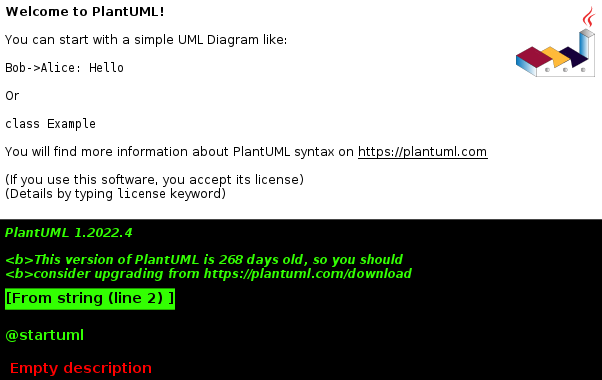
\includegraphics[width=.9\linewidth]{scheme.png}
\end{center}


\item Technology to use
\label{sec:orgc663ef8}

\begin{itemize}
\item Google Test
\item CMake
\item Standard Library For Threads (STL)
\end{itemize}
\end{enumerate}
\end{enumerate}
\end{enumerate}
\end{enumerate}


\section{Related topics}
\label{sec:org0440cfd}
\begin{itemize}
\item \href{https://epub.jku.at/obvulihs/download/pdf/6196854?originalFilename=true}{Thesis} on the use of work-stealing applied to garbage collection. In this
thesis they mention how to implement Garbage Collector Garbage First (G1)
in the HotSpot virtual machine of the Open JDK.
\end{itemize}

\section{Links}
\label{sec:org03c4346}
\begin{enumerate}
\item Philosophy
\label{sec:orge02f783}

\begin{itemize}
\item \href{https://assets.bitbashing.io/papers/concurrency-primer.pdf}{What every systems programmer should know about concurrency}
\item \href{https://www.freecodecamp.org/news/concurrency-ideologies-of-programming-languages-java-c-c-c-go-and-rust-bd4671d943f/}{Concurrency ideologies of programming languages (Java, C\#, C, C++, Go and Rust)}
\end{itemize}

\item Courses
\label{sec:org4d321a7}
\begin{itemize}
\item \href{https://ocw.mit.edu/courses/find-by-topic/\#cat=engineering\&subcat=computerscience\&spec=algorithmsanddatastructures}{Cursos MIT CS}
\item
\end{itemize}

\item Programming Languages\hfill{}\textsc{cpp:java:rust}
\label{sec:orgad203b3}
\begin{enumerate}
\item C/C++/Java
\label{sec:org7ad0358}
\begin{itemize}
\item \href{https://www.linuxjournal.com/article/6700}{Cross-Platform Software Development Using CMake}
\item \href{https://atomheartother.github.io/c++/2018/07/12/CPPDynLib.html}{Writing a cross platform dynamic library}
\item \href{https://www.quora.com/Why-is-C-faster-than-Java-1}{Why is C faster than Java?}
\item \url{https://trucosinformaticos.wordpress.com/2010/05/02/por-que-usar-const-en-c/}
\item \href{https://stackoverflow.com/questions/42310768/segmentation-fault-due-to-free-or-malloc}{Segmentation fault due to malloc or free}
\item \href{https://stackoverflow.com/questions/15604127/do-a-getter-for-an-object}{Do a geter for an object}
\item \href{https://google.github.io/googletest/}{Google tests}
\item \href{https://groups.google.com/g/comp.lang.c++.moderated/c/EA3TJcbZ73c/m/QfVUa73nwbgJ}{Is all this fancy C++ stuff used in the real world?}
\item \href{https://gitlab.com/CLIUtils/modern-cmake/-/tree/master/examples/extended-project}{extended project cmake}
\item \href{https://cliutils.gitlab.io/modern-cmake/}{Modern Cmake}
\item \href{https://github.com/Pipe-Runner-Lab/sample\_cmake}{Sample cmake}
\item \href{https://medium.com/@onur.dundar1/cmake-tutorial-585dd180109b}{Cmake tutorial}
\item \href{https://developer.ibm.com/articles/au-googletestingframework/}{Why use the google c++ testing framework}
\item \href{https://www.geeksforgeeks.org/stack-vs-heap-memory-allocation/}{Stack vs heap memory allocation}
\item \href{https://thecandcppclub.com/deepeshmenon/chapter-8-the-philosophy-of-generic-programming-in-c/709/}{The C and CPP Club}
\end{itemize}

\begin{enumerate}
\item STL C++
\label{sec:org91c15d4}
\begin{itemize}
\item \href{https://www.geeksforgeeks.org/vector-in-cpp-stl/}{vector}
\item \href{https://www.geeksforgeeks.org/list-cpp-stl/?ref=lbp}{List}
\item \href{https://www.geeksforgeeks.org/smart-pointers-cpp/}{Smart pointers}
\item \href{https://www.geeksforgeeks.org/memory-leak-in-c-and-how-to-avoid-it/\#:\~:text=Memory\%20leakage\%20occurs\%20in\%20C\%2B\%2B,by\%20using\%20wrong\%20delete\%20operator.}{Memory leakage}
\item \href{https://www.geeksforgeeks.org/few-bytes-on-null-pointer-in-c/}{Null pointers}
\item \href{https://www.geeksforgeeks.org/encapsulation-in-c/?ref=lbp}{Encapsulation}
\item \href{https://en.cppreference.com/w/cpp/memory/shared\_ptr}{Shared pointer}
\item \href{https://en.cppreference.com/w/cpp/memory/unique\_ptr}{unique\textsubscript{ptr}}
\item \href{https://en.cppreference.com/w/cpp/memory/weak\_ptr}{weak\textsubscript{ptr}}
\href{https://gist.github.com/Zitrax/a2e0040d301bf4b8ef8101c0b1e3f1d5}{string\textsubscript{format}}
\end{itemize}
\end{enumerate}

\item Techniques
\label{sec:org1a1d3ac}
\begin{itemize}
\item \href{https://mziccard.me/2015/05/08/modulo-and-division-vs-bitwise-operations/}{Modulo and Division vs Bitwise Operations}
\item \url{https://en.wikipedia.org/wiki/Locality\_of\_reference}
\begin{itemize}
\item Temporal locality
\item Spatial locality
\end{itemize}
\end{itemize}
\end{enumerate}

\item Others
\label{sec:orgcf48555}
\begin{itemize}
\item \href{https://ariannadanielle.com/why-you-need-a-website-how-to-create-your-own-website-in-a-day-for-free/}{Why you need a website as phd}
\end{itemize}

\item Techniques\hfill{}\textsc{cpp}
\label{sec:org579e148}
\begin{itemize}
\item \href{https://citeseerx.ist.psu.edu/viewdoc/download?doi=10.1.1.395.378\&rep=rep1\&type=pdf}{Hazard pointers: Safe memory reclamation for lock-free objects}
\item \href{https://comp.lang.cpp.moderated.narkive.com/vAi9h9q9/lock-free-programming-with-boost-shared-ptr-instead-of-hazard-pointers}{Shared pointers vs hazard pointers}
\item \href{https://arxiv.org/pdf/1910.11714.pdf}{Pointer life cycle types for lock-free data structures with memory
reclamation}
\item \href{http://www.cs.tau.ac.il/\~afek/Maged64bit-disc-2004.pdf}{Practical Lock-Free and Wait-Free LL/SC/VL}
\item \href{https://www.modernescpp.com/index.php/fences-as-memory-barriers}{Fences as memory barriers}
\item \href{http://concurrencyfreaks.blogspot.com/2016/08/hazard-pointers-vs-rcu.html}{Hazard Pointers vs RCU}
\end{itemize}
\end{enumerate}



\chapter{Notes}
\label{sec:orge5d5c21}

\section{Git}
\label{sec:orgdfdb5db}
\begin{enumerate}
\item Write git messages that your colleagues will love
\label{sec:orgc5eef26}
\begin{itemize}
\item Why git commit messages are important
\item Reading vs writing code
\item How to write good git commit messages
\item Focus on the why
\item Use imperative mood in the subject line
\item Restrict subject line length to 50 characters
\end{itemize}
\end{enumerate}


\chapter{Statistics}
\label{sec:orge036474}

\section{Temario tentativo}
\label{sec:orgd2bf35c}


\begin{itemize}
\item C01. Introducción a R.
\item C02. **Estadística Descriptiva.
\item C03. Gráficos.
\item **C04. **Probabilidad.
\item C05. Ajuste de distribuciones.
\item C06. Simulaciones.
\item C07. Pruebas de Hipxótesis e intervalos de confianza.
\item C08. ANOVA.
\item C09. Regresiones lineales.
\item C10. Regresiones múltiples.
\item C11. Regresiones logísticas.
\end{itemize}

\section{\href{https://www.youtube.com/watch?v=kS7nIEzyAcU}{Estadística para diseños experimentales}}
\label{sec:org5f86a37}

\begin{enumerate}
\item Diseño experimental
\label{sec:org43627c3}
\begin{itemize}
\item Población objetivo
\begin{itemize}
\item Control
\item Tratamiento
\item Seguimiento
\end{itemize}
\item Análisis
\begin{itemize}
\item Figuras descriptivas
\item Pruebas estadísticas
\end{itemize}
\end{itemize}

\item Distribución de frecuencias
\label{sec:org0b56748}

\begin{itemize}
\item Distribución normal
\begin{itemize}
\item 2 parámetros
\begin{itemize}
\item Promedio (mu)
\item Varianza
\end{itemize}
\item 1 o dos colas
\end{itemize}
\item Distribución t-student (Prueba t-student) Teorema de límite central
\begin{itemize}
\item 3 parámetros
\begin{itemize}
\item Promedio (mu)
\item Varianza (sigma cuadrada)
\item Grados de libertad (Tamaño de muestra)
\end{itemize}
\item Una o dos colas
\end{itemize}
\item Distribución F
\begin{itemize}
\item 2 grados de libertad
\end{itemize}
\item Distribución Chi-cuadrada (pruebas de hipótesis nula)
\begin{itemize}
\item 1 grado de libertad
\end{itemize}
\end{itemize}

\item Pruebas de hipótesis
\label{sec:org0ee08a7}

2 Hipótesis
\begin{itemize}
\item Hipótesis nula
\item Hipótesis alternativa
\end{itemize}

Valor crítica (alpha)
\begin{itemize}
\item \(\alpha = 5\%\) (cuando rechazar o no la hipótesis nula)
\end{itemize}

Valor de probabilidad (p)
\begin{itemize}
\item \(p > 0.05\)
\item \(p < 0.05\)
\end{itemize}

\item Pruebas estadísticas
\label{sec:org3fa411d}

\begin{enumerate}
\item Pruebas para dos grupos (muestras)
\label{sec:orgeaec4e8}

\begin{itemize}
\item T de student (versión paramétrica)
\begin{itemize}
\item Normalidad
\item Homocedasticidad
\item \(H_0 = \mu_1 - \mu_2 \neq 0\)
\item Estadístico \textbf{t}
\end{itemize}

\item Mann-Whitney (versión no-paramétrica)
\begin{itemize}
\item Distribución similar de ambos grupos
\item \(H_0 = mediana_1 = mediana_2\)
\item Estadistico: \textbf{U}
\end{itemize}
\end{itemize}

\item Pruebas para más de dos grupos
\label{sec:org18fc967}

\item Pruebas para variables continuas y categóricas
\label{sec:org4b7a19f}
\end{enumerate}
\end{enumerate}



\section{Estadística para ciencia de datos}
\label{sec:orgc6230ec}


\begin{enumerate}
\item Data Science
\label{sec:orgc06ced6}

\begin{itemize}
\item ¿Qué es ciencia de datos?
\item[{Minería de datos}] El conocimiento valioso se obtiene después de saber
como se comporta nuestra materia prima.
\end{itemize}

\begin{enumerate}
\item Estadística básica
\label{sec:orgeee18ef}

\begin{description}
\item[{Variable}] Características de un objeto o individuo que pueden medirse y
cuyo valor puede variar de acuerdo a la observación o registro.
\item[{Parámetros}] Resume el comportamiento general de las variables, en pocas
palabras, resume la información describe a un individuo, objeto o
situación.
\item[{Distribución}] El saber la distribución de la variable, nos permitirá
calcular la probabilidad de que la variable obtenga cierto valor o
aquellos valores que estén por debajo.
\end{description}
\end{enumerate}


\item Data Science Steps
\label{sec:org0f7c51b}

\item Main Concepts
\label{sec:orgaafb89b}

\item Match Between Statistic and Data Science
\label{sec:orgf2fda5b}
\end{enumerate}





\part{Plan last 2 semesters}
\label{sec:org477d466}

\begin{itemize}
\item[{$\square$}] Plan de experimentos para colas concurrentes
\begin{itemize}
\item[{$\square$}] Experimentos de LL/IC
\begin{itemize}
\item[{$\square$}] Cambios en el número de K
\end{itemize}
\item[{$\square$}] Experimentos sobre baskets
\item[{$\square$}] Experimentos sobre colas
\end{itemize}
\item[{$\square$}] Documento de avances semestral para evaluación por comité tutoral
\item[{$\square$}] Actualización código work-stealing en C++
\begin{itemize}
\item[{$\square$}] Implementación lock-free de hazard pointers
\item[{$\square$}]
\end{itemize}
\item[{$\square$}]

\item[{$\square$}] Plan de
\item
\end{itemize}

\part{Articles to begin with}
\label{sec:org3d571ae}

  Seed Papers
TITLE	FIRST AUTHOR	YEAR	CITED BY






The Google file system	GhemawatSanjay	2003	4980
Enhancing Productivity and Performance Portability of General-Purpose Parallel Programming	Alexandros Tzannes	2012	6
Scaling up parallel GC work-stealing in many-core environments	Michihiro Horie	2019	0
Idempotent work stealing	Maged M. Michael	2009	124
Defining Correctness Conditions for Concurrent Objects in Multicore Architectures	Brijesh Dongol	2015	12
Axioms for concurrent objects	Maurice Herlihy	1987	198
Reaching approximate agreement in the presence of faults	Danny Dolev	1986	484
The notions of consistency and predicate locks in a database system	Kapali P. Eswaran	1976	2052
Fence-free work stealing on bounded TSO processors	Adam Morrison	2014	19
Wait-free synchronization	Maurice Herlihy	1991	1918
Modeling of the Memory Management Process for Dynamic Work-Stealing Schedulers	Elena A. Aksenova	2017	6
Relaxed Queues and Stacks from Read/Write Operations	Armando Castaneda	2020	1
Concurrent reading and writing	Leslie Lamport	1977	295
Efficient Work Stealing for Fine Grained Parallelism	Karl-Filip Faxén	2010	46
On the minimal synchronism needed for distributed consensus	Danny Dolev	1983	694
Impossibility and universality results for wait-free synchronization	Maurice Herlihy	1988	229
Improving Load Balancing during the Marking Phase of Garbage Collection.	Erik Helin	2012	4
Concurrent Reading While Writing	Gary L. Peterson	1983	205
What Can Be Done with Consensus Number One: Relaxed Queues and Stacks	Armando Castaneda	2020	1
Efficient Synchronization-Free Work Stealing	Umut A. Acar	2011	2
Scheduling parallel programs by work stealing with private deques	Umut A. Acar	2013	121
Cilk: An Efficient Multithreaded Runtime System	Robert D. Blumofe	1996	1880
The structure of the “THE”-multiprogramming system	Edsger W. Dijkstra	1968	1189
How to Make a Multiprocessor Computer That Correctly Executes Multiprocess Programs	Leslie Lamport	1979	2754
Algorithms for scalable synchronization on shared-memory multiprocessors	John M. Mellor-Crummey	1991	1355
Work-Stealing for Multi-socket Architecture	Quan Chen	2017	0
Simple, fast, and practical non-blocking and blocking concurrent queue algorithms	Maged M. Michael	1996	836
Fully Read/Write Fence-Free Work-Stealing with Multiplicity	Armando Castaneda	2021	0

\part{Bibliography}
\label{sec:orge7e19a0}
\bibliographystyle{plainurl}
\bibliography{refs}
\end{document}